%% LyX 2.0.5.1 created this file.  For more info, see http://www.lyx.org/.
%% Do not edit unless you really know what you are doing.
\documentclass[10pt,twocolumn,english]{svjour3}
\usepackage[T1]{fontenc}
\usepackage[latin9]{inputenc}
\usepackage{babel}
\usepackage{amstext}
\usepackage{amsmath}
\usepackage{amssymb}
\usepackage{graphicx}
\usepackage{bm}
\usepackage{esint}
\usepackage[authoryear]{natbib}
\usepackage[unicode=true]
 {hyperref}
\usepackage{subfig}

\newcommand{\argmin}{\operatorname*{argmin}}
\newcommand{\erfi}{\operatorname{erfi}}
\newcommand{\psf}{\operatorname{PSF}}
\newcommand{\snr}{\operatorname{SNR}}

\makeatletter
%%%%%%%%%%%%%%%%%%%%%%%%%%%%%% User specified LaTeX commands.
\date{}

\makeatother

\begin{document}

\title{simpleSTORM - a Fast, Self-Calibrating Reconstruction Algorithm for
Localization Microscopy}


\author{Ullrich K{\"o}the, Frank Herrmannsd{\"o}rfer, Ilia Kats, Fred A. Hamprecht\\
Multi-Dimensional Image Processing Group, University of Heidelberg}

\maketitle

\section{Introduction}

Localization microscopy techniques such as STORM and PALM have become
major tools for cell biology \citet{bates_08_super-resolution,heilemann_10_fluorescence,henriques_09_palm-and-storm,huang_10_super-resolution}.
Despite differences in the experimental procedures, these techniques
rest on a unified computational principle: Super-resolution images
are constructed by means of subpixel-accurate spot detection in a
sequence of images taken at optical resolution. Various algorithms
have been proposed for this task and many of them are available in
open-source software. We will briefly review existing algorithms below.

While many existing algorithms are in principle able to obtain good
reconstructions, practical success requires a careful adjustment of
various configuration settings. This parameter tuning may be difficult
even for experts and raises the entry threshold for localization microscopy
novices. To overcome this problem, simpleSTORM was designed to determine
all necessary parameters automatically from the raw image data itself
during an initial \emph{self-calibration phase} that precedes the
actual reconstruction phase. It can thus produce good reconstructions
with virtually no user input, while still allowing optional configuration
by experts for non-standard use cases.

simpleSTORM is based on an accurate model of the image acquisition
process. It assumes that photon counting noise is the dominant noise
source and follows a Poisson distribution. However, photon counts
are not directly observed, but are transformed by various amplification
stages and digitization. We assume that the combined transformation
can be described by a linear equation. Poisson-distributed intensities
can thus be recovered by inverting this linear equation, provided
its parameters (gain and offset) are known. Furthermore, we assume
that the point spread function (PSF) is a Gaussian with unknown (but
fixed) width. Finally, we assume that the background intensity varies
at a much coarser scale than the PSF and that less than half of the
pixels in any sufficiently large window contain signal. Under these
assumptions, the model parameters (gain and offset, PSF width, local
background intensity) can be estimated automatically in a self-calibration
and preprocessing phase.

In the reconstruction phase, the model parameters are used to transform
each frame such that it can be considered as a sum of background-free
fluorescence signal and additive Gaussian noise with zero mean and
unit variance. Fluorescence spots can thus be recognized by a simple
statistical test: A pixel whose intensity is higher than three times
the noise standard deviation contains signal with a probability of
about 99.7\% (the threshold of the test can be adjusted to control
the detection sensitivity of our algorithm). Since the PSF spreads
over several pixels, whereas the noise of neighboring pixels is independent,
it is even more unlikely that three adjacent pixels exceed the threshold
just by chance. The combination of both criteria defines a reliable
mask for spot detection. Pixels under (and near) the mask are finally
convolved with a matched filter (i.e. a Gaussian filter corresponding
to the PSF) for optimal noise reduction and interpolated to the desired
resolution using a cubic spline. The coordinates of local intensity
maxima after interpolation are reported as the detected spots.

\noindent \newpage{}Specifically, the algorithm proceeds in these
steps:
\begin{enumerate}
\item Robust estimation of the gain and offset parameters
\item Estimation of the width of a Gaussian PSF via the power spectrum
\item Linear intensity transform into unit gain and zero offset to make
the noise approximately Poisson distributed 
\item Anscombe transform of the intensities to make the noise approximately
normal
\item Dynamic background estimation and subtraction
\item Statistical test to determine the detection mask according to the
specified sensitivity
\item Matched filtering with the PSF for optimal noise reduction
\item Cubic spline interpolation to specified subpixel accuracy and maxima
detection
\end{enumerate}
On a standard laptop, our algorithm is able to process about 20 frames
per second for a typical raw image size of 200x200 pixels. It performed
favorably in the recent ISBI Localization Microscopy Challenge (\href{http://bigwww.epfl.ch/smlm/challenge/}{bigwww.epfl.ch/smlm/challenge/})
that carefully tested more than 20 reconstruction algorithms. In particular,
simpleSTORM achieved high localization accuracy on high-density data,
where a relatively large number of spots was simultaneously switched
on in order to minimize total acquisition time. Software for our algorithm
is freely available in an easy-to-use GUI program at \href{https://github.com/ukoethe/simple-STORM}{github.com/ukoethe/simple-STORM}.

\begin{figure*}
\begin{centering}
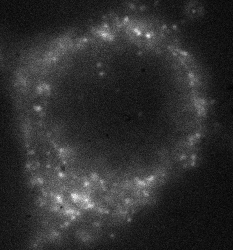
\includegraphics[width=0.45\textwidth]{figures/RawImage}$\qquad$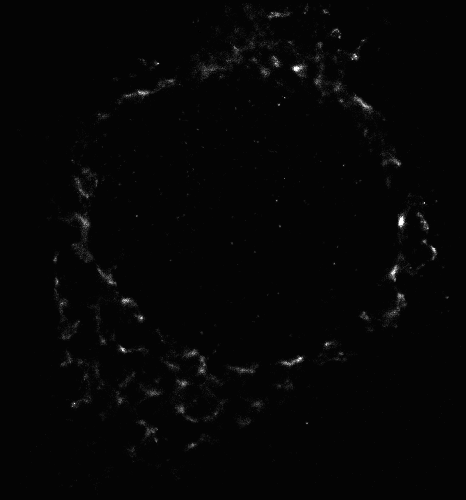
\includegraphics[width=0.45\textwidth]{figures/reconstructedImage}
\par\end{centering}

\caption{Example result from simpleSTORM (data courtesy of Mike Heilemann).
Left: one frame of the raw data. Right: reconstructed high-resolution
image.}


\end{figure*}



\section{Related Work}

The classical reconstruction approach is based on direct fitting of
the PSF to every spot candidate. A model of the PSF with adjustable
parameters must be given. Usually, an isotropic Gaussian PSF like
(\ref{eq:gaussian-psf}) or an anisotropic variant of it is sufficiently
accurate \cite{thompson_02_precise}. The free parameters of the
model are optimized by a non-linear fitting algorithm (e.g. the Levenberg-Marquart
method) in order to minimize the least-squares residual between the
fitted model and the intensities of a spot candidate. This method is the basis of the 
popular rapidSTORM software \cite{wolter_10_rapid-storm}, the ImageJ plugins PeakFit \cite{herbert_12_peakfit}, GrapsJ (offering GPU accelaration) \cite{brede_12_graspj} and Octane \cite{yu_11_octane}, as well as the Localization Microscopy MicroManager plugin \cite{stuurman_12_plugin} and PYME (the Python localization microscopy environment) \cite{baddeley_12_pyme}.

An even simpler approach avoids iterative optimization by computing the centroid of 
each spot directly, either in terms of the intensity-weighted mean \cite{thompson_02_precise} or the 
fluoroBancroft method \cite{andersson_08_localization}. These methods were found to be only 
slightly less accurate then the least-squares fit when properly parameterized \cite{thompson_02_precise,hedde_09_localization-microscopy} and form the basis of fast reconstruction solutions such as the hardware-accelerated method of \cite{gruell_11_fpga-storm} and the QuickPALM ImageJ plugin \cite{henriques_10_quick-palm}.

Both fitting and direct methods have difficulties with the reconstruction of high density image sequences, because these images violate the basic model assumption that neighboring spots do not overlap. Greedy procedures to fit overlapping spots where proposed by \cite{egner_07_nanoscopy}, who adapt H{\"o}gbom's classical CLEAN algorithm \cite{hoegbom_74_clean} to localization microscopy, the DAOSTORM algorithm from \cite{holden_11_daostorm}, an adaptation of DAOPHOT, a well-known algorithm from astronomy \cite{stetson_87_daophot}, and the multi-emitter fitting algorithm of \cite{huang_11_simultaneous}, who fit up to $N_{\max}$ overlapping PSFs simultaneously and select the most likely spot number by a statistical test. A more principled model for overlapping spots is provided by {\em compressed sensing} \cite{zhu_12_faster-storm}. Here, a PSF candidate is initialized at all pixels of a fine grid (e.g. having one-eighth the pixel size of the original image). The fit is then performed under a strong {\em sparsity prior} which ensures that only the center pixels of true spots get non-zero activation. While this method is more accurate than DAOSTORM, it is also very expensive (about a hundred times slower). Recently, substantial improvements of the sparse reconstruction approach have been achieved by more sophisticated modeling and optimization methods \cite{kim_13_localization-microscopy,min_13_localization-microscopy}. 

Proper noise modeling is a critical ingredient for reliable distinction between true spot and noise artefacts. Many authors simply use a generic additive noise model and select spots whose intensity exceeds the background by a certain multiple of the background's noise standard deviation \cite{thompson_02_precise,gruell_11_fpga-storm}. Frequently, the image is preprocessed by averaging filters \cite{wolter_10_rapid-storm,huang_11_simultaneous}, Gaussian filters \cite{krizek_11_minimizing} or a wavelet transform \cite{izeddin_12_wavelet} before thresholding. However, non-uniform background intensity and intensity-dependent background noise  make the choice of an appropriate threshold very difficult. Heuristic solutions to this problem lead to algorithms with many adjustable parameters that are very hard to use.

Moreover, it has been shown in \cite{abraham_09_localization-estimation} that a maximum likelihood fit based on a Poisson noise model outperforms the least-squares algorithm which implicitly assumes additive noise. A fast GPU-accelarated version of this method is described in \cite{smith_10_fast}. However, the Poisson model cannot be applied directly to the observed image intensities because they differ from the Poisson-distributed photon counts by various aplification steps and are no longer Poisson distributed. The amplification can be inverted when gain factor and offset are known, but this requirement is apparently overlooked sometimes (e.g. \cite{andersson_08_localization,gruell_11_fpga-storm,brede_12_graspj}). A simple gain and offset estimation procedure using dedicated calibration images was proposed in \cite{lidke_05_photon-statistics}. A more convenient self-calibration algorithm was introduced in \cite{boulanger_10_patch-based}, who adaptiveliy subdivide the real images to determine regions of homogeneous intensity for gain estimation. This method is very similar in spirit to our approach in section \ref{sec:noise-normalization}, but their algorithm is considerably more complicated.

\section{Methods}

\subsection{\label{sec:matched-filters}Matched Filters}

Many existing reconstruction algorithms determine spot positions by
fitting a PSF model to the intensities in suitable candidate regions.
Under certain conditions, an equivalent effect can be achieved in
a simpler and numerically more robust way by means of \emph{matched
filters} \citet{turin_60_matched-filters}. We briefly recall the
underlying theory. Let the image $s(x,y)$ contain just a single spot
at an unknown location $(x_{0},y_{0})$. Since the image is corrupted
by noise, we cannot simply detect the spot by looking for the point
of maximum intensity in $s$. To simplify matters, we assume that
the noise is additive Gaussian noise with zero mean and variance $\sigma^{2}$,
i.e. our image model is
\begin{eqnarray}
s(x,y)=\psf(x-x_{0},y-y_{0})&+&n(x,y) \label{eq:simple-signal-model} \\ && n(x,y)\sim\mathcal{N}(0,\sigma^{2}) \nonumber
\end{eqnarray}
We now seek a filter function $h(x,y)$ such that filtering of $s$
with $h$ maximizes the signal-to-noise ratio of the filtered image
$g(x,y)=g_{\psf}(x,y)+g_{n}(x,y)$. The signal and noise parts
of the filtered image are given by the convolution integrals
\begin{eqnarray*}
g_{\psf}(x,y) & = & h\star\psf \\ &=&\int_{\mathbb{R}^{2}}h(x',y')\,\psf(x-x',y-y')\, dx'\, dy'\\
g_{n}(x,y) & = & h\star n \\ &=&\int_{\mathbb{R}^{2}}h(x',y')\, n(x-x',y-y')\, dx'\, dy'
\end{eqnarray*}
Signal and noise energies are defined by the squares of these expressions.
Since the noise is, by assumption, uncorrelated with the filter, the
noise energy simplifies to $g_{n}(x,y)^{2}=\sigma^{2}\int_{\mathbb{R}^{2}}h(x',y')^{2}\, dx'\, dy'$
according to Parseval's theorem. The signal-to-noise ratio (SNR) at a point
$(x,y)$ is the quotient of the corresponding energies, i.e.
\[
\snr(x,y)=\frac{\left(\int_{\mathbb{R}^{2}}h(x',y')\,\psf(x-x',y-y')\, dx'\, dy'\right)^{2}}{\sigma^{2}\int_{\mathbb{R}^{2}}h(x',y')^{2}\, dx'\, dy'}
\]
The energy of the PSF is given by 
\begin{eqnarray*}
E_{\psf}&=&\int_{\mathbb{R}^{2}}\psf(x',y')^{2}\, dx'\, dy'\\ &=&\int_{\mathbb{R}^{2}}\psf(x-x',y-y')^{2}\, dx'\, dy'
\end{eqnarray*}
where the second identity follows from translation invariance. We
can therefore rewrite the SNR as
\begin{multline*}
\snr(x,y)=\frac{E_{\psf}}{\sigma^{2}} \cdot\\
\quad\,\,\frac{\left(\int_{\mathbb{R}^{2}}h(x',y')\,\psf(x-x',y-y')\, dx'\, dy'\right)^{2}}{\int_{\mathbb{R}^{2}}h(x',y')^{2}\, dx'\, dy'\int_{\mathbb{R}^{2}}\psf(x-x',y-y')^{2}\, dx'\, dy'}
\end{multline*}
The second quotient is easily recognized as the square of the correlation
coefficient $\rho$ between the filter $h$ and the mirrored PSF.
We must therefore maximize the correlation coefficient in order to
maximize the SNR for given signal and noise energy. The correlation
coefficient assumes its highest possible value $\rho=1$ when 
\[
h(x,y)=\kappa\,\psf(-x,-y)
\]
for any $\kappa\ne0$. In other words, the filter should have the
same shape as the signal we want to detect, but mirrored at the origin.
The convenient choice $\kappa=1$ results in the \emph{matched filter},
which is thus optimal under the model of additive Gaussian noise.
The spot is localized at the point where the filter result $g=h\star s$
assumes its local maximum. This location can be determined by spline
interpolation of $g$, see section \ref{sec:spot-localization}.

To use matched filters in localization microscopy, the following requirements
must be met:
\begin{enumerate}
\item The PSF must be known. We address this in section \ref{sec:psf-estimation}.
\item The PSF should be uniform throughout the image. This condition may
not be fulfilled when some spots are out of focus. However, this is
not a major problem in practice, because the filter $h$ degrades
gracefully: Although no longer the best possible filter, it still
performs reasonably as long as the PSF is not too far off. 
\item Each image should contain only one spot. This is clearly violated
in practice and in fact undesirable. But this is not a serios problem
either as long as the spot density is not too high. Since the PSF
decreases quickly, the filter response at point $(x,y)$ is not influenced
by spots that are sufficiently far away. The detector suffers only
a minor degradation in localization performance at overlapping spots
when their distance remains larger than the PSFs full width at half
maximum (FWHM). The spot density can easily be controlled by the experimental
setup.
\item The image's background intensity must be zero. We use a standard background
subtraction procedure as described in section \ref{sec:background-subtraction}.
\item The noise must be additive Gaussian. This is the most serious obstacle,
because the noise level actually depends on the intensity and is therefore
not additive. To rescue the matched filter approach, we transform
the original image intensities so that the noise is approximately
turned into additive Gaussian noise. Our \emph{noise normalization}
procedure is described in section \ref{sec:noise-normalization}.
\end{enumerate}

\subsection{\label{sec:noise-normalization}Noise Normalization}

Matched filtering is only optimal when the noise is additive and Gaussian
distributed. However, localization microscopy is based on a photon
counting process, which instead follows a Poisson distribution with
intensity-dependent variance. The probability of observing $k$ photons
in pixel $(x,y)$ when the expected count (i.e. the true intensity)
is $\lambda=\lambda(x,y)$ is given by
\[
p\left(k\right)=\frac{\lambda^{k}}{k!}e^{-\lambda}
\]
(we dropped the dependency on $(x,y)$ to improve readability). Moreover,
these counts are not observed directly but are subjected to several
amplification stages and discretized into a finite set of gray levels.
If we assume linear amplification characteristics and neglect discretization
effects%
\footnote{This is possible because the discretization noise is much smaller
than the noise from other sources in a well-calibrated setup.%
}, the observed image gray levels $k'$ depend on $k$ according to
the linear function 
\[
k'=a\, k+b
\]
where $a$ denotes the combined amplification factor and $b$ the
dark signal. The noise in $k'$ is no longer Poisson distributed.
One can easily see this by recalling that both the mean and variance
of a Poisson distribution are equal to $\lambda$. In contrast, mean
and variance of $k'$ are
\begin{eqnarray*}
E\left[k'\right] & = & a\, E\left[k\right]+b=a\,\lambda+b\\
Var\left[k'\right] & = & a^{2}\, Var\left[k\right]=a^{2}\lambda
\end{eqnarray*}
and these quantities are in general different. Figure ??? illustrates
the difference between the distributions of $k$ and $k'$ for a representative
choice of $\lambda$, $a$, and $b$. Consequently, it is \emph{incorrect}
to apply algorithms (e.g. matched filtering) directly to the observed
image $k_{t}'(x,y)$ at time step $t$ when these algorithms rest
on the assumption of either Gaussian or Poisson noise. Fortunately,
there is an easy way out: the \emph{Anscombe transform \citet{anscombe_48_noise-normalization}}
\[
q_{t}(x,y)=2\sqrt{k_{t}(x,y)+\frac{3}{8}}
\]
turns a Poisson distributed signal $k_{t}(x,y)$ into an approximately
Gaussian distributed one $q_{t}(x,y)$ with unit variance, regardless
of the value of $k$ (as long as $k\ge4$). However, in order to apply
the Anscombe transform, we need to know the coefficients $a$ and
$b$ that map the observed gray values $k'$ back into the Poisson
distributed counts $k$:
\begin{equation}
q(x,y)=2\sqrt{\frac{k'(x,y)-b}{a}+\frac{3}{8}}\label{eq:anscombe-transform}
\end{equation}
Dermining $a$ and $b$ turns out to be a difficult problem. The standard
solution is to record dedicated calibration images where the mean
and variance of $k'$ can be computed easily. Then, a linear regression
through a set of pairs $\left(E[k'],\, Var[k']\right)$ with different
$k'$ directly provides the desired coefficients. However, this approach
is inconvenient when the camera is mounted on a microscope, and it
must be repeated whenever any camera or amplifier settings change.
Therefore, we seek to determine these coefficients by self-calibration,
i.e. from the raw localization images themselves. 

Among a large number of ideas we tried, the following turned out to
be the most stable. Consider a pixel $(x,y)$ whose gray value is
constant over time, i.e. the pixel contains background or a bead,
but no blinking molecule. Then we can easily compute its average intensity
and variance over time and obtain a pair for the linear regression.
The difficulty is that we do not know which pixels have this property.
The following consideration shows a way to identify them: Whenever
the true intensity is not constant, the apparent variance is larger
than it would otherwise be, because
\[
Var\left[f(t)+n(t)\right]=Var\left[f(t)\right]+Var\left[n(t)\right]
\]
where $f(t)$ is a time-dependent signal and $n(t)$ denotes noise
which is uncorrelated with the temporal behavior of $f$. When $f(t)$
is actually constant over time, its variance is zero, resulting in
the minimal possible value of $Var\left[f(t)+n(t)\right]$. Otherwise,
this value always increases. This leads to the following algorithm
\begin{enumerate}
\item Select $n$ image locations at random.
\item Compute mean and variance of the corresponding pixels over the first
$T$ frames of the sequence ($T=200$ works well in practice, but
the value can be adjusted). Create the scatter plot of the resulting
mean/variance pairs.
\item Use the RANSAC algorithm to compute the lower leaning line of the
scatter plot: Repeat $k=???$ times:

\begin{enumerate}
\item Select two points at random and compute the line through these points.
\item Determine the number of inliers of this line, i.e. the number of points
whose distance from the line is at most ???.
\item Keep the line with the maximum number of inliers as the best estimate
of the lower leaning line.
\end{enumerate}
\item The coefficients $a$ and $b$ now correspond to the slope and intercept
of the lower leaning line, because this line contains precisely the
points whose intensity was constant over time. All points not near
the lower leaning line are ``contaminated'' by intensity variations
and therefore ignored. 
\end{enumerate}
\begin{figure}
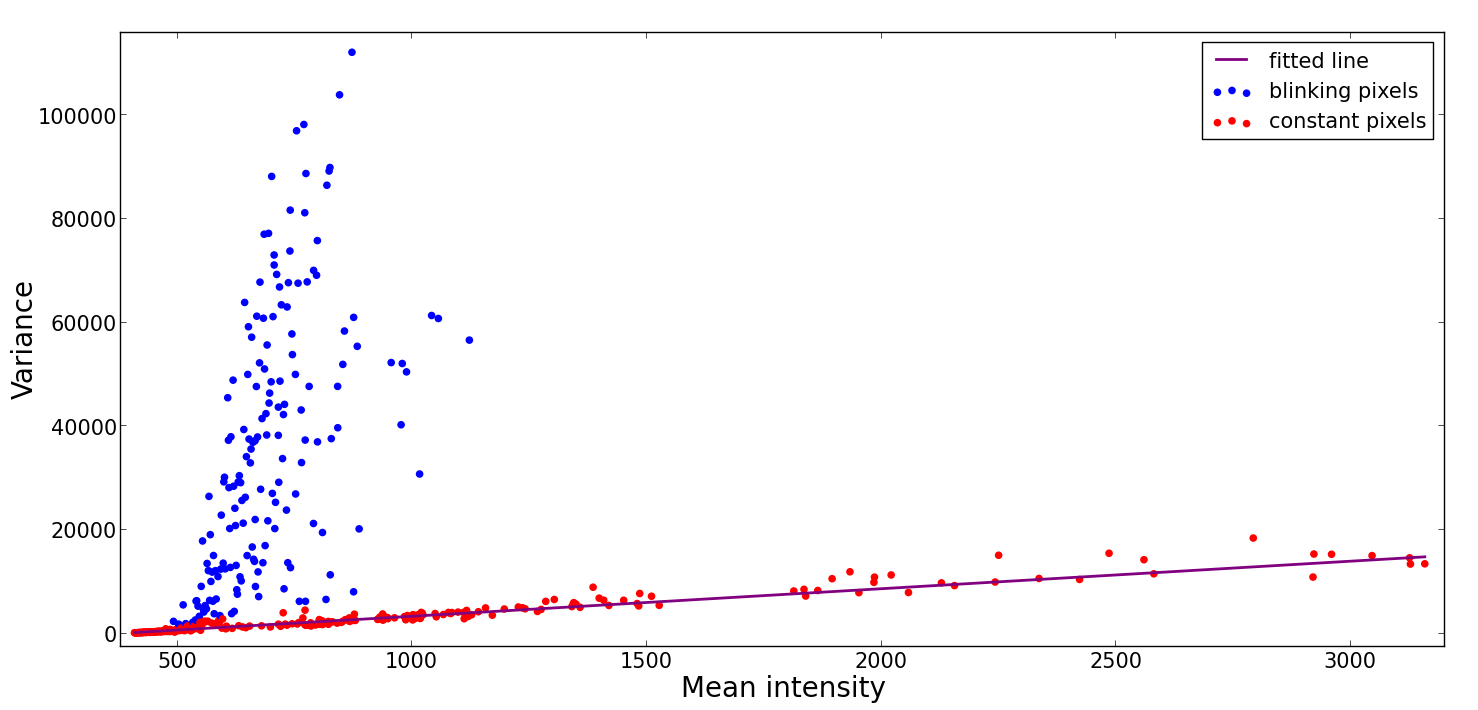
\includegraphics[width=1\columnwidth]{figures/lower-leaning-line}

\caption{\label{fig:lower-leaning-line}RANSAC-fitting of a lower leaning line
to a scatter plot showing variance vs. mean intensity for randomly
selected pixels. Slope and intercept of this line determine the correction
coefficients in equation (\ref{eq:anscombe-transform}).}


\end{figure}
Figure \ref{fig:lower-leaning-line} shows two examples of the fit
according to this algorithm. It can be seen that it does indeed detect
the lower leaning line of the scatter plot, which corresponds to the
pixels with constant intensity.

Explain the post-optimization of a and b for unit variance???


\subsection{\label{sec:background-subtraction}Background Subtraction}

Once the noise model is known, we transform the observed images $k_{t}'(x,y)$
into noise-normalized ones $q_{t}(x,y)$ according to (\ref{eq:anscombe-transform})
and subsequent local optimization???. The next step is the estimation
of the background intensity. It is based on the standard assumption
that thes background intensity varies mauch slower then the actual
signal both spatially and over time. We split the dataset into non-overlapping
blocks of size $\rho^{2}\times\tau$, where $\rho$ is the block size
in the two spatial directions, and $\text{\ensuremath{\tau}}$ is
the block size along the time direction. Default values of $\rho=30$
and $\tau=20$ work well in all our experiments. If necessary, the
user can adjust these settings. This is easy because the she can determine
how fast the background varies by simple visual inspection of the
data. 

In each block, the median of the gray values $s$ is computed. The
median is preferrable to the mean because it is more stable when the
block contains non-background pixels (blinking spots and beads): These
pixels lead to a significant upward bias in the mean, whereas the
median increases only marginally. The meadian values are placed on
the grid defined by the centers of the blocks, and interpolated to
the original image resolution (both in spatial and time direction)
using a Catmull-Rom spline which ensures smooth (i.e. differentiable)
interpolation and thus avoids blocking artifacts in the background
estimate $\beta_{t}(x,y)$. After subtracting $\beta_{t}$ from the
noise normalized signal $q_{t}$, we obtain the signal $s_{t}$ which
has unit variance in all pixels and zero mean in the background:
\begin{equation}
s_{t}(x,y)=q_{t}(x,y)-\beta_{t}(x,y)\label{eq:background-subtraction}
\end{equation}
The images $s_{t}$ now conform to the requirements of the matched
filter method, which relies on the noise being additive with constant
variance and the background being zero. Figure \ref{fig:background-subtraction}
shows an example.

\begin{figure*}
\begin{center}

\includegraphics[width=0.4\textwidth]{figures/Tubulin2OrigFrame50}$\qquad$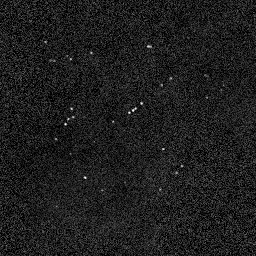
\includegraphics[width=0.4\textwidth]{figures/Tubulin2normalprocessFrame50}
\end{center}
\caption{\label{fig:background-subtraction}Left: original image (frame 50
of the Tubulin2 dataset more???). Right: the same frame after noise
normalization and background subtraction according to equations (\ref{eq:anscombe-transform})
and (\ref{eq:background-subtraction}).}


\end{figure*}



\subsection{\label{sec:psf-estimation}Estimation of the PSF}

In order to apply the matched filter method, the PSF must be known.
Accurate PSF estimates are crucial for the matched filter to perform
optimally. We investigated two approaches to PSF estimation, a non-parametric
and a parametric one. In both cases, the PSF is estimated by averaging
over the response of many spots in order to get rid of the noise. It should also be noted that we estimate $\sigma_{\psf}$ after noise normalization and background subtraction. This estimate is related to the PSF size $\sigma^*_{\psf}$ in the raw data by the relation $\sigma_{\psf}=\sqrt{2}\,\sigma^*_{\psf}$.

The non-parametric method estimates the PSF in the form of an optimal
\emph{Wiener filter} which is based on the \emph{magnitude spectrum}
of the signal. Let
\[
S_{t}=\mathcal{F}[s_{t}]
\]
the Fourier transform of frame $s_{t}$ (after noise normalization
and background subtraction). Then the average power spectrum over
T frames is
\[
P=\frac{1}{T}\sum_{t=1}^{T}\left|S_{t}\right|^{2}
\]
where $\left|S_{t}\right|$ is the point-wise magnitude of the complex
frequency response. The Wiener filter is then defined as
\[
W=\left(\frac{P-P_{N}}{P}\right)_{+}
\]
where $P_{N}$ is the expected power spectrum of the noise and $\left(.\right)_{+}=\max\left(0,.\right)$
is the hinge function that truncates negative values at zero (negative
values can occur because we estimate $W$ from only finitely many
frames). Since the noise is (thanks to noise normalization and background
subtraction) additive Gaussian noise with zero mean and unit variance,
its expected power spectrum is simply $P_{N}=1$. The matched filter
can now be computed by multiplication of each frame's Fourier transform
with the Wiener filter, followed by inverse Fourier transform
\[
\hat{s}_{t}=\mathcal{F}^{-1}[S_{t}\cdot W]
\]
In contrast, the parameteric method assumes that the PSF is shaped
like a Gaussian, which is a very good approximation for typical microscopes.
Under this assumption, the self-calibration only needs to determine
a single parameter, the PSF scale. Clearly, the variance of a single
parameter estimate is much smaller than the variance of an entire
non-parametric PSF estimate from the same number of samples. The Gaussian
model is therefore preferable when it conforms to the actual PSF shape,
whereas deviations between model and real PSF will lead to noticeable
bias in spot localization. 

The Gaussian fit can be performed both in the spatial and in the Fourier
domain. The Fourier domain approach starts in the same way as in the
non-parametric case, i.e. we compute the average power spectrum of
the noise-normalized signal. To simplify subsequent computations,
we cut out $T'$ sufficiently large square ROIs from the original
frames and compute their average power spectrum $P'$. Now, instead
of using the power spectrum directly to define a Wiener filter, we
compute the average magnitude spectrum $\sqrt{P'}$ and use it to
fit a Gaussian function. Since the Fourier transform of a Gaussian
PSF and the corresponding magnitude spectrum are again rotationally
symmetric Gaussian functions, the model is 
\begin{equation}
g(r | w_1, w_2, w_3) = w_{1}\,\exp\left(-\frac{r^{2}}{2w_{2}^{2}}\right)+w_{3}\label{eq:gaussian-psf}
\end{equation}
where $r=\sqrt{u^{2}+v^{2}}$ is the distance of the point from the
origin. The parameters $w_{i}$ are choosen by means of non-linear
least-squares optimization (typically using the Levenberg-Marquardt algorithm) such that
the squared difference between the model and the power spectrum is
minimized
\[
w_{1},w_{2},w_{3}=\argmin_{w_{i}}\sum_{u,v}\left[g(r | w_1, w_2, w_3)-\sqrt{P'(r)}\right]^{2}
\]
Parameters $w_{1}$ and $w_{3}$ account for the signal and noise
intensities respectively, whereas the desired PSF scale in the spatial
domain can be obtained from the parameter $w_{2}$ be the simple relation
\[
\sigma_{\psf}=\frac{W}{2\pi w_{2}}
\]
where $W$ is the width of the ROI used to compute the magnitude spectrum
(recall that we select squared ROIs to simplify matters). The fit
in the spatial domain is performed similarly, but the simple averaging
via the average power spectrum is not possible here. Instead, we fit
the PSF independently to a number of easy-to-detect spots, and than
define $\sigma_{\psf}$ as the median of the parameter $w_2$ of the individual estimates.
Finally, the result of matched filtering is 
\[
\hat{s}_{t}=s_{t}\star\mathrm{gauss}_{\sigma_{\psf}}
\]
where $\star$ denotes convolution.

Experiments reported in section ??? reveal that the parametric estimate
is usually superior to the non-para\-metric one, confirming that the
Gaussian model is indeed feasible in practice. Moreover, it turns
out that the spatial domain estimate is better because ???.


\subsection{Spot Detection}

After the self-calibration phase, the actual data processing starts.
Now, the parameters estimated during calibration are used to preprocess
every frame of the sequence. Spot detection is performed after noise
normalization and background subtraction according to equations (\ref{eq:anscombe-transform})
and (\ref{eq:background-subtraction}). Since the background contains
now only Gaussian additive noise with zero mean and unit variance,
a standard statistical test can be used to detect pixels whose intensity
is unlikely to be background. For a given $p$-value, corresponding
to the probability of false positives, the intensity threshold is
\[
t\ge\sqrt{2}\,\erfi(2p-1)
\]
where $\erfi(.)$ is the inverse error function. That is, a
normalized pixel with intensity at least $t$ has a probability of
at most $p$ to represent background. For example, $p$-values of
1\% and 0.1\% correspond to thresholds 2.3 and 3.1 and indicate that
one gets one false positive on average per 10x10 and 30x30 window
respectively. Note that these thresholds are independent of the image
content. Thanks to noise normalization and background subtraction,
there is no need for manual threshold adjustment or complicated threshold
selection heuristics.

Nonetheless, the error rate is still rather high, but further increases
of the threshold are undesirable because this would reduce the sensitivity
of the detector for true positives. However, we can still do better
by noticing that true spots cover several pixels (according to the
width of the PSF), whereas the noise of neighboring pixels is uncorrelated.
Therefore, the probability that multiple adjacent are above threshold
\emph{simultaneously} is much lower for background pixels, whereas
this event is very probable for a true spot. In practice, we accept
a spot if at least three connected pixels exceed the threshold for
the chosen $p$-value. The probability of false positives in this
setting can be approximated by a binomial distribution with parameter
$p$. For example, for $p=1\%$, the probability that three or more
background pixels are above threshold in a given 3x3 window is only
$0.01\%$ (one false positive in every 100x100 window), for $p=0.1\%$
the resulting probability is $10^{-5}\%$. This approximation slightly
over-estimates the accuracy of our algorithm because the approximation
assumes that 3x3 windows are independent which is clearly not true
for overlapping windows. However, experiments show that the false
positive rate (number of false positives over total number of background
pixels) is indeed very low, namely 228 false positives out of 46 million for $p=1\%$ and 16 for $p=0.1\%$, see section ??? for details.
The result of this step is a set of spot masks, i.e. connected regions
above threshold that contain at least three pixels.


\subsection{\label{sec:spot-localization}Spot Localization}

In order to perform spot localization, we first subject the normalized
image to the matched filter described in section \ref{sec:matched-filters},
i.e. we filter with a Gaussian whose size $\sigma_{\psf}$ has
been determined according to section \ref{sec:psf-estimation}. We
don't apply this filter before spot \emph{detection} because this
would introduce complicated correlation between the noise of neighboring
pixels, making the differentiation between signal and noise more difficult. 

The theory of matched filtering suggests that each local maximum of
the filtered image corresponds to a location of best match between
the data and the spot model. This location needs to be determined
to subpixel accuracy, and a residual error of 1/10 of a pixel is typically
achievable. The simplest possibility to do so is via cubic spline
interpolation of the filtered image to the desired resolution. The
upsampling ratio can be chosen by the user and is typically between
8 and 16. To save time, the interpolation is only performed in sufficiently
large rectangles around each spot mask (i.e. the bounding rectangle
plus ??? pixels in every direction). Each local maximum of the interpolated
image which is covered by one of the spot masks is returned as a detected
spot. 

Important spot properties such as signal-to-noise ratio and anisotropy
can be readily obtained from the properties of the interpolated image.
Let $g$ be the intensity of the interpolated image at the local maximum
position, and $g_{xx}$, $g_{xy}$, $g_{yy}$ the corresponding second
derivatives (these derivatives can be easily computed analytically
from the spline representation). Then the following relations can be derived from basic properties of Gaussian functions. Since the noise has unit variance before matched filtering, the (unfiltered) signal-to-noise ratio is simply
given by  
\[
\snr=2g
\]
(the factor of 2 accounts for the smoothing effect of the matched
filter). The standard deviation of the 2D localization error $\Delta \bm{x}$ in units of the pixel spacing is then
\begin{equation}
\mathrm{StdDev}[\Delta \bm{x}]=\frac{1}{g \sqrt{\pi}}\label{eq:spot-std-dev}
\end{equation}
This is of the expected form, because $g$ is proportional to $\sqrt{N}$ (the square root of the photon count) due to the action of the Anscombe transform.

The maximum and minimum radius of a potentially unisotropic spot can be computed from the eigenvalues
of the second derivative matrix
\[
\kappa_{1,2}=\frac{1}{2}\left(g_{xx}+g_{yy}\pm\sqrt{g_{xx}^{2}+g_{yy}^{2}+4\, g_{xy}^{2}-2\, g_{xx}g_{yy}}\right)
\]
by the expressions
\begin{eqnarray*}
s_{\max} & = & \sqrt{-g/\kappa_{1}-\sigma_{\psf}^{2}}\\
s_{\min} & = & \sqrt{-g/\kappa_{2}-\sigma_{\psf}^{2}}
\end{eqnarray*}
and their ratio gives the spot anisotropy

\[
\mbox{AI}=\frac{s_{\max}}{s_{\min}}
\]
Spot radii and anisotropy can serve as additional selection criteria
to remove undesired anisotropic spots, or as a means to determine
spot depth in 3D localization microscopy with cylindrical lenses.

It should be noted that each spot mask can contain multiple local
maxima. This is desirable because it allows us to detect overlapping
spots, provided that the overlap is not too big. Specifically, overlapping
spots of equal intensity remain separable (i.e. give rise to distinct
maxima) when their centers have a distance of more than $2\sqrt{2}\,\sigma_{\psf}$.
This is an advantage of the matched filtering method over reconstruction
algorithms that directly fit the PSF to the image data: The fitting
approach only works reliably when the spots do not overlap significantly,
i.e. when the spot distance is about twice as big.


\section{Results}
\subsection{Validation}
For validation purposes the trainings datasets released for the ISBI Single-Molecule Localization Microscopy Challenge 2013 were used as well as the evaluation tool.\newline
There are four different datasets. Two datasets with simulated tubulin tubes, we will refer to these datasets as tubulin 1 and tubulin 2 dataset. The tubulin 1 and tubulin 2 dataset consist of  2400 frames and simulated autofluorescent background. The tubulin 2 dataset has the same structure as tubulin 1 dataset but a higher level of noise.\newline
The other two datasets simulated a bundle of tubulin tubes. There is a long sequence set with 12000 frames and almost no overlapping PSF and a high density set with 361 frames and frequently overlapping PSFs. Both datasets will be referred to as long sequence dataset and high density dataset respectively. 
\subsection{PSF width estimation}
As described above the performance of the matched filter depends on the proper estimation of the PSF width. For SimpleSTORM the Levenberg-Marquardt algorithm was chosen to estimate the PSF width, since it performs almost as good as the matched filter determined from the power spectrum but gives the opportunity to set the PSF width manually. For data with a high density of fluorophores there is a trade-off between the increasing localization accuracy and the chance of near PSFs merge into one due to filtering. This effect is shown in Figure \ref{sigmas} which shows how the reconstruction gets worse with higher filter width. The same effect of merging PSFs and decreasing localization accuracy is also shown in Figure \ref{sigmas_quantitativeA}. Both Figures are based on the reconstruction of the same image, which was processed with the same parameters except the filter width. From left to right the filter width increases. Two effects are visible, the decrease of the number of localizations and the loss of structural information. The true PSF width is approximately 1 pixel in the raw images.  Although the appropriate filter width was used in the second picture of Figure \ref{sigmas}, the filtering did not perform best. This shows that in case of high PSF density it can be favorable to use a smaller filter to avoid merging PSFs. Figure \ref{sigmas_quantitativeB} shows that for high density datasets it is even more favorable to use a smaller filter width instead of the true PSF width.
The estimation of the PSF width using the Fourier transformed imaged proved to be not reliable. It tended to overestimate the true PSF width.

\begin{figure}
\subfloat[$\sigma = 0$]{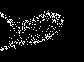
\includegraphics[width = 0.15\textwidth]{figures/bundledTubulins2_sigma_0_croped.png}}\hfill%
\subfloat[$\sigma = 1$]{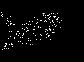
\includegraphics[width = 0.15\textwidth]{figures/bundledTubulins2_sigma_1_croped.png}}\hfill%
\subfloat[$\sigma = 1.5$]{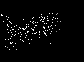
\includegraphics[width = 0.15\textwidth]{figures/bundledTubulins2_sigma_1_5_croped.png}}\hfill%
	\caption{The effect of different filter widths on datasets with a high PSF density per frame.}%
	\label{sigmas}%
\end{figure}

\begin{figure}
\subfloat[Long sequence dataset]{
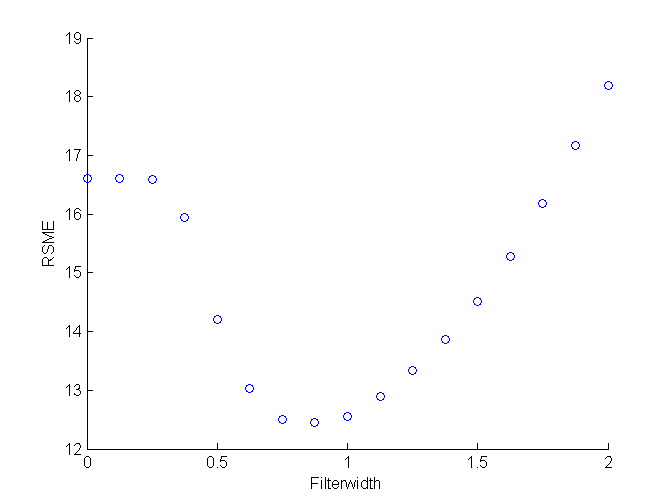
\includegraphics[width=0.22\textwidth]{figures/RMSEoverFilterwidth.png}\label{sigmas_quantitativeA}}\hfill%
\subfloat[High density dataset]{
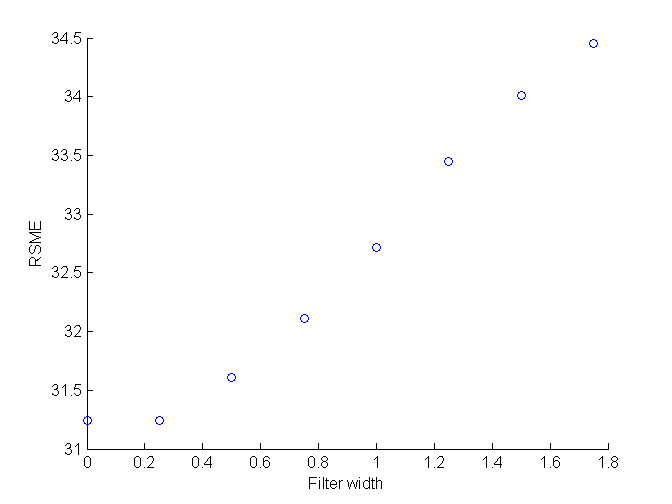
\includegraphics[width=0.22\textwidth]{figures/RMSEoverFilterwidth_hd.png}\label{sigmas_quantitativeB}}
	\caption{RSME for different filter widths.}%
	\label{sigmas_quantitative}%
\end{figure}



To validate the PSFs width estimation using the Levenberg-Marquardt algorithm all PSFs from the first 2000 frames (all frames from high density dataset) of the datasets provided from the ISBI challenge were detected and fitted. Figure \ref{histogram_of_sigmas} shows the distribution of the estimated width in histograms. The calculated values for the training datasets are 109~nm which means 1.09 pixels for the high density and long sequence dataset and 0.73 pixels respectively. The estimated PSF width lies within a then percent range according to the calculated on. The only exception is the high density dataset for which the PSF width is overestimated because of the many overlapping PSFs.

\begin{figure}
\subfloat[Long sequence dataset, true sigma is 1.08]{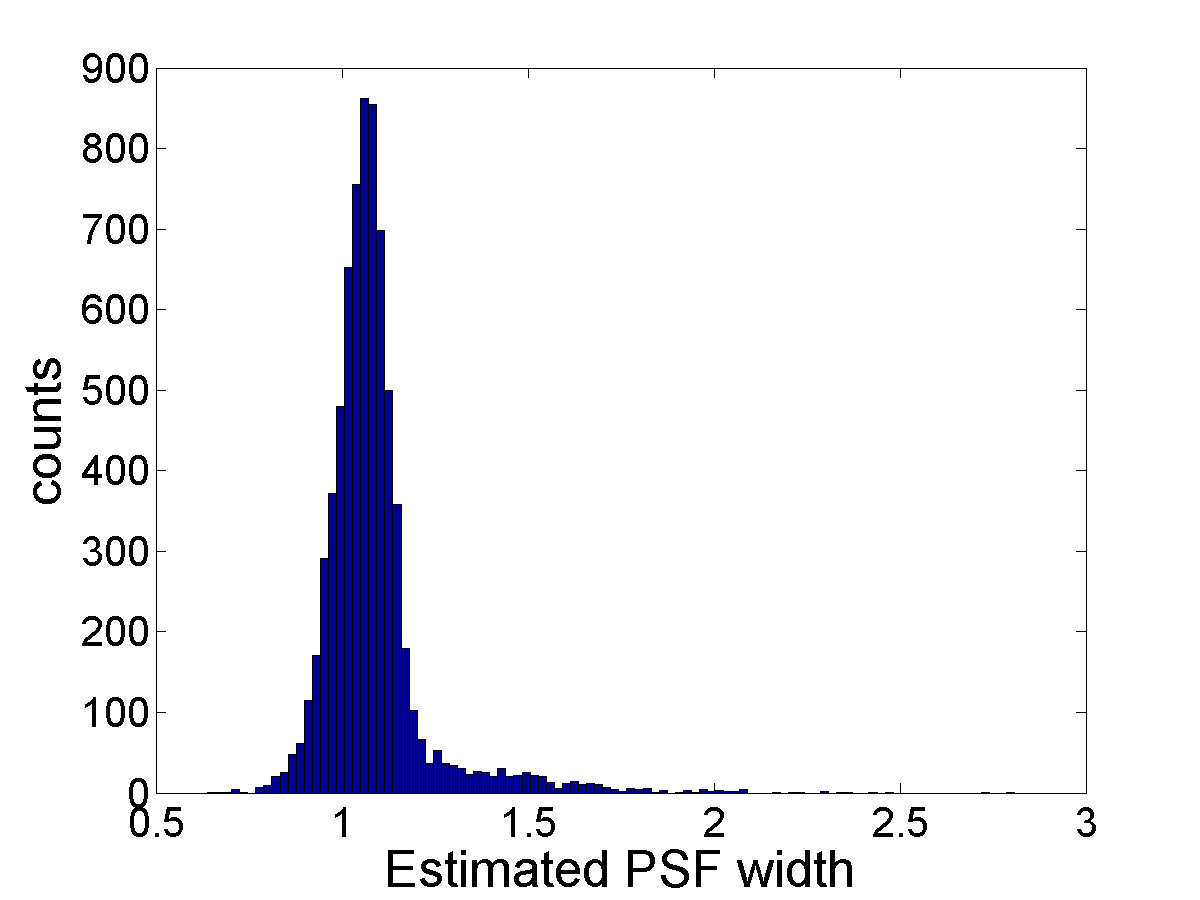
\includegraphics[width = 0.24\textwidth]{figures/SigmaBundledTubes1.png}}\hfill%
\subfloat[High density dataset, true sigma is 1.08]{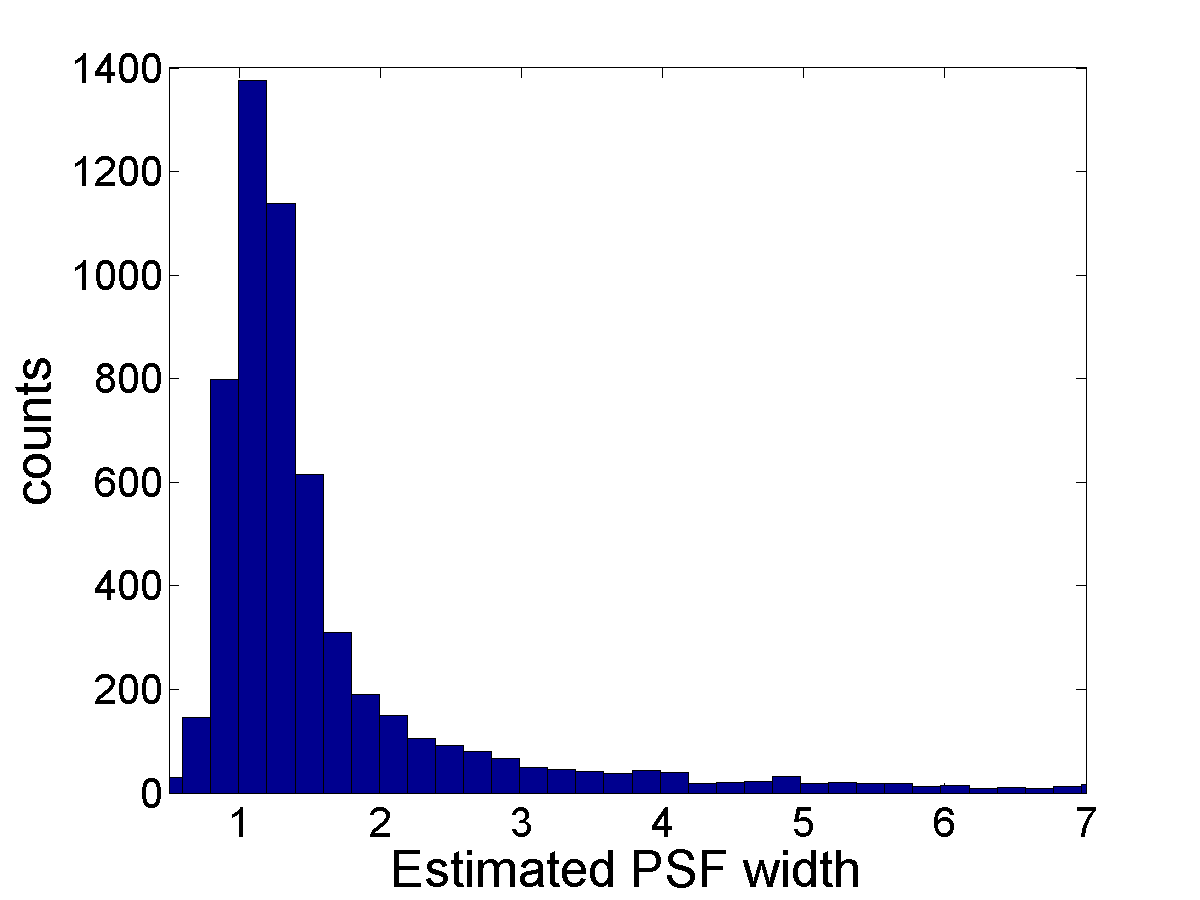
\includegraphics[width = 0.24\textwidth]{figures/SigmaBundledTubes2.png}}\hfill%
\subfloat[Tubulin 1 dataset, true sigma is 0.8]{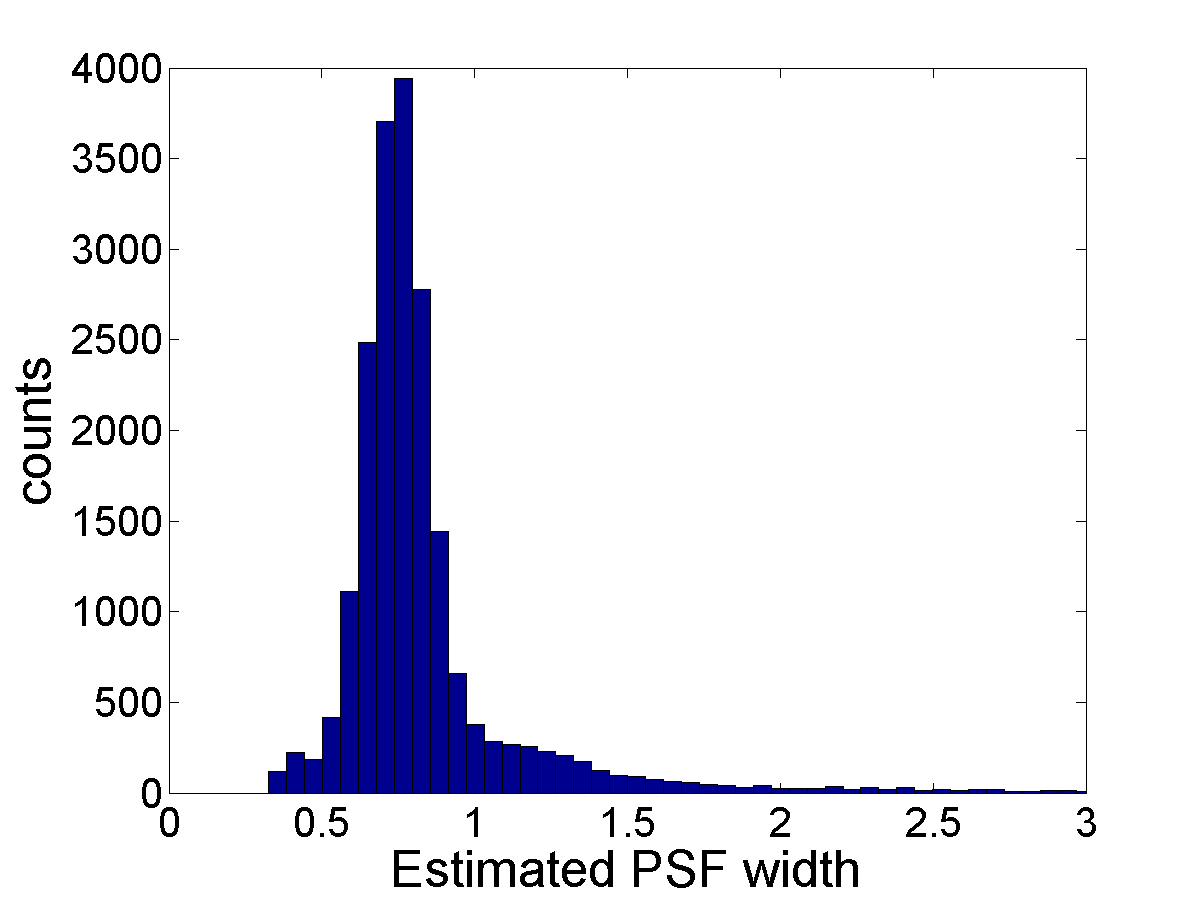
\includegraphics[width = 0.24\textwidth]{figures/SigmaTubulin1.png}}\hfill%
\subfloat[Tubulin 2 dataset, true sigma is 0.8]{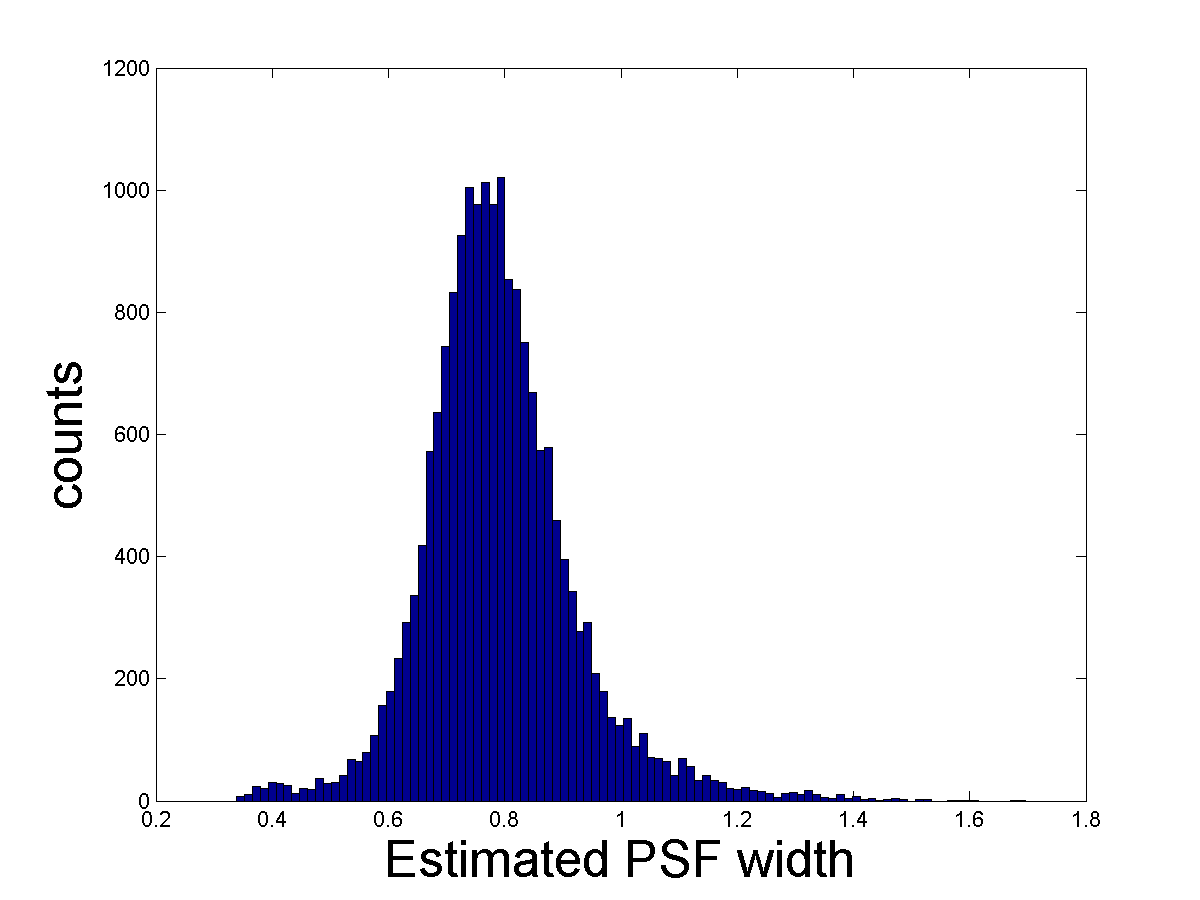
\includegraphics[width = 0.24\textwidth]{figures/SigmaTubulin2.png}}
	\caption{Histograms for three training datasets from the ISBI localization challenge}%
	\label{histogram_of_sigmas}%
\end{figure}

\subsection{Gain estimation}
One key feature is the estimation of the camera gain directly from the data. This is important since the actual gain factor differs from the set one. For validation purpose a series of 500 frames of an average cell culture sample with phalloidin labeled actin filaments were captured several times with different gain settings. Figure \ref{gain_verification} shows the linear relation between the estimated gain factor and the set one.

\begin{figure}
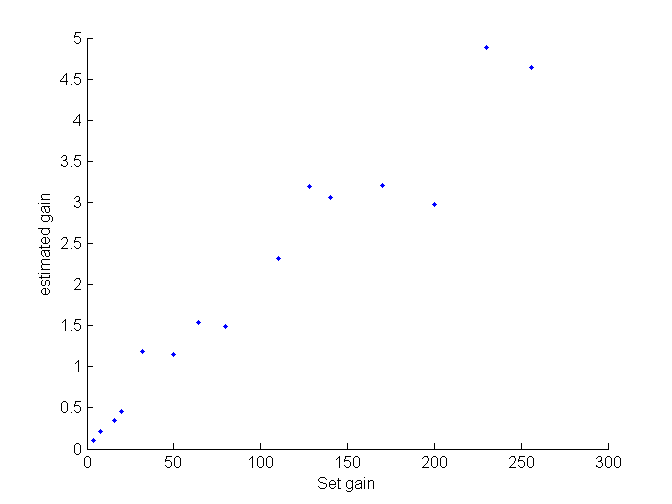
\includegraphics[width=0.45\textwidth]{figures/gain_estimation}
\caption{Scatter plot of estimated gain over set gain. The same sample was imaged multiple times with different gain factors set in the camera settings.}
\label{gain_verification}
\end{figure}

\subsection{Background estimation}
To check whether the background estimation and Anscombe transformation worked as supposed, the false positive to background pixel rate was determined. The $p-$value determines the rate of false positives per background pixels. The number of background pixels that are erroreously detected as signal was calculated for the training datasets of the ISBI challenge. For each frame the background subtraction and the Anscombe transformation was applied and the number of background pixels were counted that exceed the threshold corresponding to different $p$-values. This rate of false positives to background pixels can be seen in Figure \ref{fp_rate}. The more important error rate is calculated from the pixels that exceed the threshold and have two neighbors that exceed the threshold too. This rate over the corresponding $p$-value is shown in Figure \ref{fp3_rate}.

\begin{figure}
\subfloat[False positive to background pixel rate.]{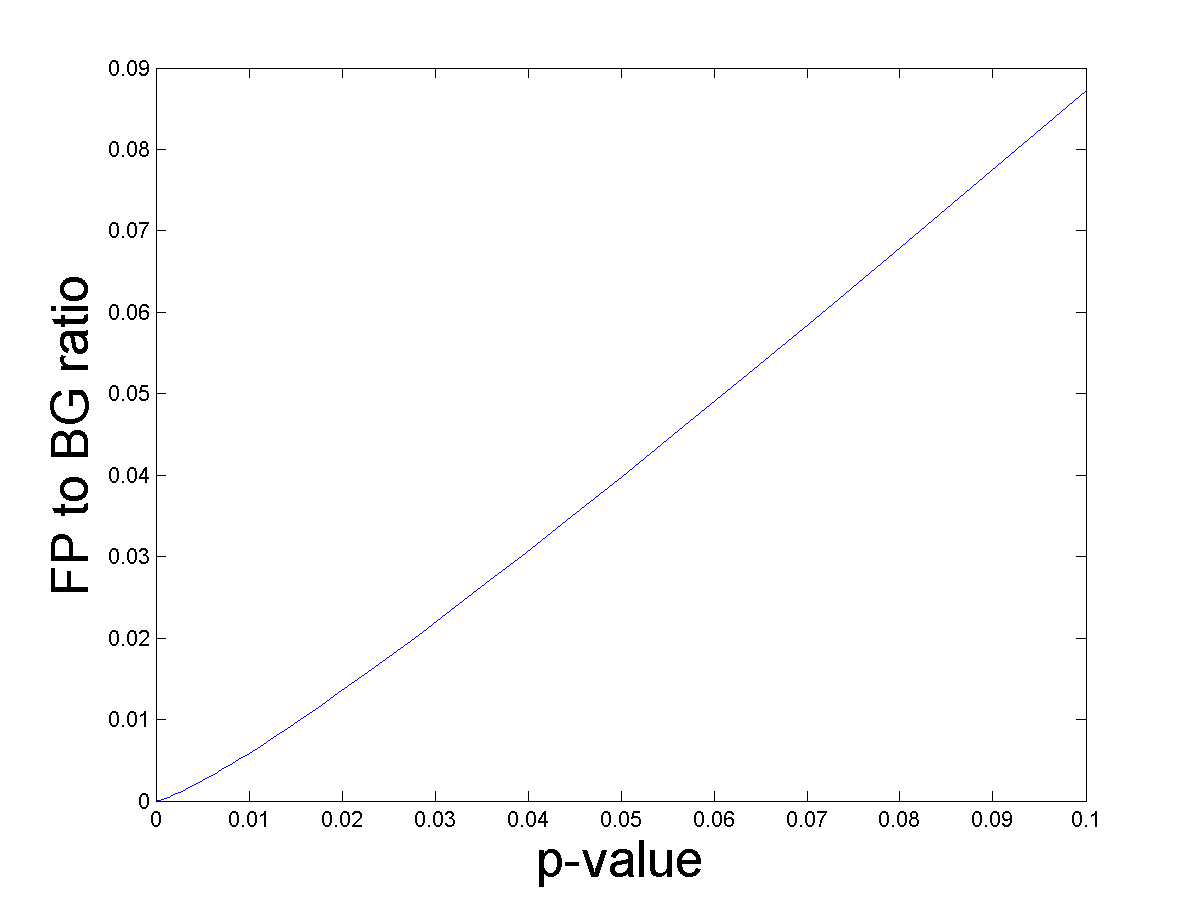
\includegraphics[width = 0.24\textwidth]{figures/FP_BgRatioTubulin1.png}\label{fp_rate}}\hfill%
\subfloat[False positive rate only considering false positives with at least 2 neighbours.]{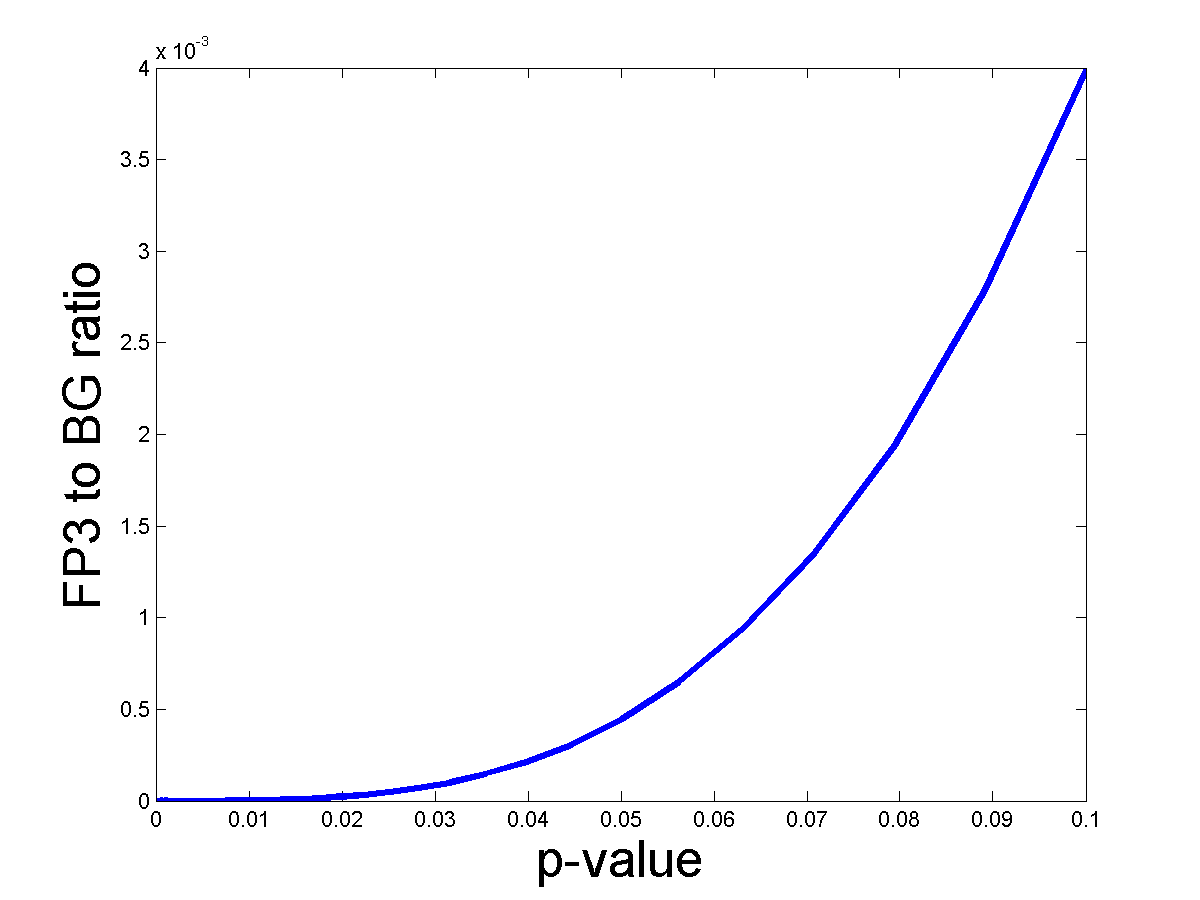
\includegraphics[width = 0.24\textwidth]{figures/FP3_BgRatioTubulin1.png}\label{fp3_rate}}\hfill%	
\caption{False positives rates.}%
\end{figure}

\subsection{Results on the trainings datasets}
No parameter has to be set to produce reasonable results using SimpleSTORM. However advanced users can adjust the settings to optimize the output according to the total number of fluorophores detected or the RSME or something in between. It is not possible to optimize Jaccard index and RSME at the same time. 
SimpleSTORM gives the opportunity to set the p-value, an asymmetry threshold and the upscaling factor. Table \ref{improvements} shows the changes for Jaccard index, f-score and RSME for the long sequence dataset evaluated for a lateral tolerance of 50~nm which corresponds to half of the width of the raw image. Baseline settings are, camera parameters automatically detected,  p-value = 0.1~\%, upscale factor = 10 and asymmetry threshold off.
\begin{table}
\caption{Effect of different settings.}
\begin{tabular}{l|ccc}
&Jaccard&f-score&RSME\\\hline
baseline&0.824&0.903&12.88\\
p-val = 0.001~\%&0.815&0.898&12.76\\
asymmetry (1.5)&0.620&0.765&12.13\\
upscale factor = 100&0.619&0.764&11.45
\end{tabular}
\label{improvements}
\end{table}
Lowering the p-value does not alter the results significantly. The reason is that even for the baselines p-value, almost no false positives are detected. Applying an asymmetry threshold discards many true positives but also improves the localization error due to the selection the best and undisturbed PSFs. A higher upsampling factor increases the localization accuracy without removing any points but increasing the reconstruction time.\newline

To give an objective impression of the SimpleSTORM algorithm the four training datasets are processed with the standard parameters except the upscaling factor. Gain offset and PSF width were estimated from the data and the standard p-value of 0.0001 (0.01~\%) was used. For evaluation of the results the evaluation tool available on the ISBI challenge website was used. Table \ref{result_Training_0_3} shows the results for Jaccard index, f-score, precision and RSME. For the evaluation only ground truth localizations within a lateral tolerance disk around the detected molecule positions are considered. Thus the radius of the lateral tolerance disk is crucial for the results. The radius was set at a rate of 0.3 the pixel size of the raw data. The RSME is given in nanometers.
%\begin{table}
%\caption{Radius 0.1}
%\begin{tabular}{l|ccccc}
%&Jaccard&F-Score&Precision&RSME\\ \hline
%Tubulin1&0.261&0.414&0.630&9.19\\
%Tubulin2&0.126&0.224&0.508&9.64\\
%LS&0.442&0.613&0.669&6.154\\
%HD&0.007&0.013&0.094&7.038
%\end{tabular}
%\label{result_Training_0_1}
%\end{table}

\begin{table}
\caption{Radius 0.3}
\begin{tabular}{l|cccccc}
&Jaccard&Precision&RSME&time in sec.\\ \hline
Tubulin1&0.437&0.936&15.7&55.9\\
Tubulin2&0.232&0.904&18.8&46.2\\
LS&0.761&0.946&9.97&50.1\\
HD&0.031&0.449&20.55&7.2
\end{tabular}
\label{result_Training_0_3}
\end{table}

%\begin{table}
%\caption{Radius 0.5}
%\begin{tabular}{l|ccccc}
%&Jaccard&F-Score&Precision&RSME\\ \hline
%Tubulin1&0.470&0.640&0.974&19.6\\
%Tubulin2&0.270&0.426&0.966&22.9\\
%LS&0.805&0.892&0.974&11.6\\
%HD&0.060&0.112&0.788&32.168
%\end{tabular}
%\label{result_Training_0_1}
%\end{table}

%\begin{table}
%\caption{Radius 1}
%\begin{tabular}{l|ccccc}
%&Jaccard&F-Score&Precision&RSME\\ \hline
%Tubulin1&0.487&0.655&0.997&26.6\\
%Tubulin2&0.282&0.439&0.997&31.0\\
%LS&0.836&0.911&0.994&15.7\\
%HD&0.075&0.139&0.976&55.1
%\end{tabular}
%\label{result_Training_1}
%\end{table}



\section*{Acknowledgement}

This research was supported by contract research ``Methoden f{\"u}r die Lebenswissenschaften'' of the Baden-W{\"u}r\-ttemberg Stiftung.

\bibliographystyle{spbasic}
\bibliography{simpleSTORM}

\end{document}
